\documentclass{report}
\usepackage[margin=1in]{geometry} 
\usepackage{amsmath,amsthm,amssymb,amsfonts}
\usepackage{tabto}
\usepackage[yyyymmdd]{datetime}
\renewcommand{\dateseparator}{--}
\newcommand{\N}{\mathbb{N}}
\newcommand{\Z}{\mathbb{Z}}

% For definitions
%\newtheorem{defn}{Definition}[section]
%\newtheorem{thrm}{Theorem}[section]
%\newtheorem{ex}[Example}[section]
\newtheorem*{ex}{Example}
\newtheorem*{defn}{Definition}
\newtheorem*{thrm}{Theorem}
\newtheorem*{lemma}{Lemma}
\newtheorem*{result}{Result}

% For circled text
\usepackage{tikz}
\newcommand*\circled[1]{\tikz[baseline=(char.base)]{
            \node[shape=circle,draw,inner sep=0.8pt] (char) {#1};}}

\usepackage{pgf}
\usetikzlibrary{arrows, automata}

% For equation system alignment
\usepackage{systeme,mathtools}
% Usage:
%	\[
%	\sysdelim.\}\systeme{
%	3z +y = 10,
%	x + y +  z = 6,
%	3y - z = 13}

\newenvironment{problem}[2][Problem]{\begin{trivlist}
\item[\hskip \labelsep {\bfseries #1}\hskip \labelsep {\bfseries #2.}]}{\end{trivlist}}
%If you want to title your bold things something different just make another thing exactly like this but replace "problem" with the name of the thing you want, like theorem or lemma or whatever
 
%used for matrix vertical line
\makeatletter
\renewcommand*\env@matrix[1][*\c@MaxMatrixCols c]{%
  \hskip -\arraycolsep
  \let\@ifnextchar\new@ifnextchar
  \array{#1}}
\makeatother 
 
% Change chapter numbering
\newcommand{\mychapter}[2]{
	\setcounter{chapter}{#1}
	\setcounter{section}{0}
	\chapter*{#2}
	\addcontentsline{toc}{chapter}{#2}
}

\usepackage{graphicx}
\graphicspath{ {images/} }

\begin{document}
 
\tableofcontents{}
\mychapter{1}{2018-01-30}
\section{Depth First Search (DFS)}
\begin{defn}
For graph $G$:\\
You start with $S$ and try first edge leading to $V$. Then you follow the first edge leading out of $V$. Continue like this until you reach a dead end. Then backtrack until you get to node with an unvisited node.
\end{defn}
\subsection{BFS vs DFS}
Similarities:
	\begin{itemize}
	\item Cross through all the nodes.
	\item Similar level of efficiency.
	\end{itemize}
Differences:
	\begin{itemize}
	\item Ordering of nodes are very different.
	\end{itemize}

\subsection{DFS (u)}
	\begin{verbatim}
	Mark u as explored and add u to R
	Foreach edge (u,v) incident to v
	  IF v is not marked as explored then
	    recursively invoke DFS(v)
	  Endif
	Endfor
	\end{verbatim}

\subsection{Adjacency Matrix/ Adjacency List}
Matrices are nice for understanding graphs but they aren't nice for implementing them since they use space $O(n^2)$.\\
\begin{ex}
Given we have $n$ vertices and $m$ edges:\\
Adjacency matrix has space complexity of $O(n+m)$ when given a sparse graph meaning the number of edges is not much larger than the number of nodes. Since there are $n+m$ representations of the graph, then going through the structure (identifying all edges) will also take $O(n+m)$ time.
\end{ex}
\begin{ex}
Given a matrix with N=100 items and a cost of $c$. Then the max cost is $100c$.\\
Then the number of elements in the list will be 100 and the time to traverse the list will be $100c$ in other words $(n+m)c$ where $(n+m)$ is the entire representation of the graph.
\end{ex}

Adjacency List needs $O(n+m)$ space for sparse graphs.
\begin{enumerate}
\item Array Adj where Adj[v] is a record containing the list of all nodes adjacent to $v$.
\item For undirected graph $G(V,E)$ each edge $e(v,w)$ occurs on two adjacency lists: node w appears on the list for node $v$, node $v$ appears on the list for node $w$.
\item Need an array of pointers of length n to setup list in Adj; we need the space for all the lists.
\item Length of the list may vary but in (1) and (2) $e(v,w)$ appears in exactly two of the lists: One for $v$ and one for $w$. Thus the total length of all the lists is $2m$. \qed
\end{enumerate}
Best case space complexity for list is $\Omega(n)$, worst case is $O(n^2)$ for when graph is complete, and average case is $\Theta(m+n)$.\\
BFS Traversal is $O(n+m) = O(n^2)$.

\mychapter{2}{2018-02-06}
\section{Topological Sorting}
\subsection{Sorting Directed Acyclic Graph}
\begin{thrm}
If $G$ has a topological ordering then $G$ is a DAG (Directed Acyclic Graph).\\
The converse is also true. So if $G$ is a DAG, then $G$ has a topological order.
\end{thrm}
\begin{ex}
Below is a directed acyclic graph $G$ and its topological sorting.
\begin{center}
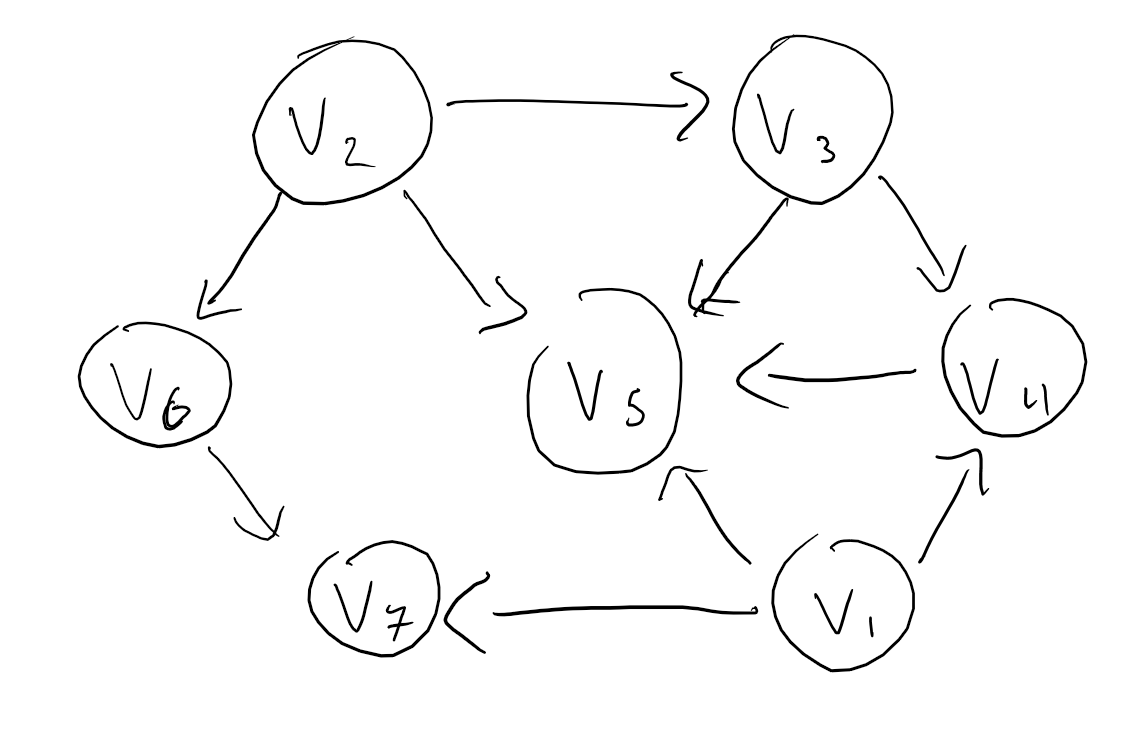
\includegraphics[scale=0.5]{TopSortingGraph1.png}\\
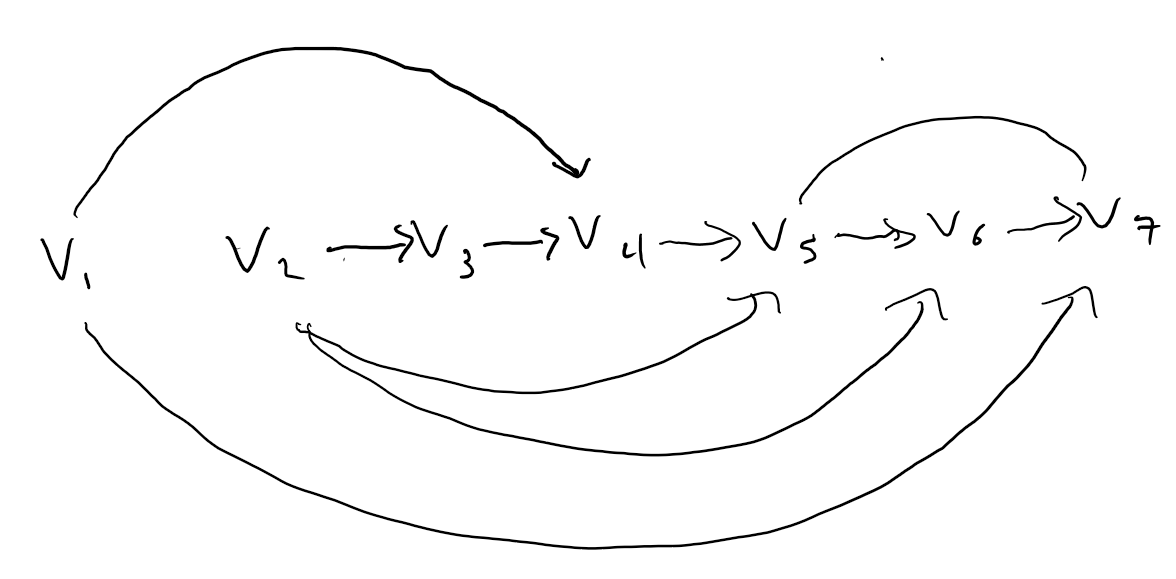
\includegraphics[scale=0.5]{TopologicalSorting1.png}
\end{center}
\end{ex}
Testing graph functions in \LaTeX
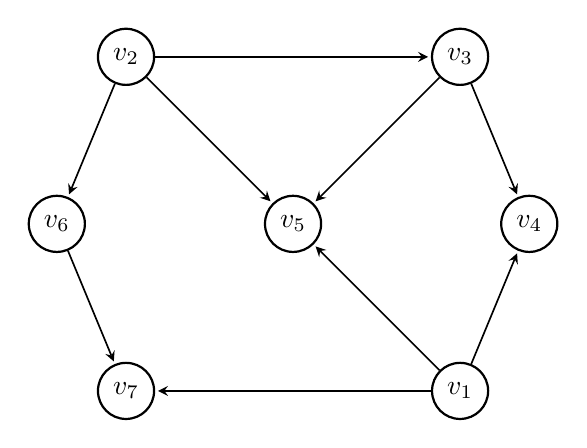
\begin{tikzpicture}[> = stealth,shorten > = 1pt,auto,node distance = 3cm,semithick]
\tikzstyle{every state}=[draw = black,thick,fill = white,minimum size = 4mm]
	
	\node[state] (v5) {$v_5$};
	\node[state] (v7) [below left of=v5] {$v_7$};
	\node[state] (v4) [right of=v5] {$v_4$};
	\node[state] (v6) [left of=v5] {$v_6$};
	\node[state] (v2) [above left of=v5] {$v_2$};
	\node[state] (v3) [above right of=v5] {$v_3$};
	\node[state] (v1) [below right of=v5] {$v_1$};
	
	\path[->] (v1) edge node {} (v4);
	\path[->] (v1) edge node {} (v7);
	\path[->] (v1) edge node {} (v5);
	\path[->] (v2) edge node {} (v6);
	\path[->] (v2) edge node {} (v5);
	\path[->] (v2) edge node {} (v3);
	\path[->] (v3) edge node {} (v5);
	\path[->] (v3) edge node {} (v4);
	\path[->] (v6) edge node {} (v7);
\end{tikzpicture}

\subsection{Divide and Conquer}
Divide and Conquer is a strategy of solving problems by splitting a task into smaller pieces and working on each piece individually.\\
This system also allows us to merge the pieces back together in linear time.\\
\subsection{Insertion Sort}
Step or moment of key:\\
$\Theta(N)$ steps in terms of key positions = $\Theta(N)$ time.
$\Theta(N^2)$ time.\\
Can we make this algorithm better than $\Theta(N^2)$?

\mychapter{3}{2018-02-13}
\section{Counting Inversions}
\begin{problem}\\
We are given n numbers $\{a_1,a_2,...,a_n\}$. We want to define a measure that tells us how far this list is from being in ascending order.
\end{problem}
\begin{ex}
Given a list $\{2,4,1,3,5\}$. We want to find how far this list is from $\{1,2,3,4,5\}$ In other words, how many of the numbers in the first list are out of order.\\
Starting from the left of the first list 2 is less than 4 so it is in order but 4 is greater than 1 so that is out of order. So the number of inversions for this list is $(2,1)$, $(4,1)$, $(4,3)$.\\
Naive Algorithm: Each pair $(a_i,a_j)$ and determine whether it constitutes an inversion. $O(n^2)$.\\
Better solution:
\begin{enumerate}
\item Divide the list into two pieces $\{a_1,...,a_m\}$ and $\{a_{m+1},...,a_n\}$
\item Count the inversions in each half separately.
\item Count the number of inversions of both halves combined.
\end{enumerate}
$T(n) \leq 2T(\frac{n}{2})+cn \rightarrow O(n\log(n))$
Algorithm:
\begin{enumerate}
\item Recursively sort first and second half and count the number of inversions in each half.
\item We now have two sorted lists $A$ and $B$ containing the first and second half.
\item Create single sorted list $C$ while counting the number of compares that are inverted.
\end{enumerate}
Counting the Inversions:
\begin{enumerate}
\item Because $A$ and $B$ are sorted, every time $a_i$ is appended to $C$ no new inversions are encountered because $a_i$ is smaller than all of the elements in $B$.
\item Every time $b_j$ is appended to list $C$ then it is smaller than all of the elements in $A$. Then the number of inversions that will be counted would be the number of elements recursively in $A$.
\item Counting line $i$.
\end{enumerate}
So when you're merging the two remaining lists together, you compare item by item. Which ever item is smaller than the other means that that item is smaller than every item in the other list. So if you have two lists of length five, on the first comparison, which ever item is smaller gets put into the final list and the number of inversions is incremented by five. You only count these inversions for one list however. So if you choose list $B$ to be the inversion counter, then any time an item in $A$ is smaller, the number of inversions doesn't go up.\\
At any point in this merge, when an element in the inversion counting list is smaller than the comparison element in the other list, the inversion count goes up by however many items are remaining in the other list.\\ 
\end{ex}

\mychapter{4}{2018-02-15}
\section{Quicksort}
Quicksort is a divide and conquer style algorithm.
\subsection{Algorithm}
Quicksort follows the following steps:
\begin{enumerate}
\item Select an element of the array. This will be our 'pivot'.
\item Partition the remaining elements to two groups:\\
$S_1 = \{x\in S - \{v\} | x\leq v\}$\\
$S_2 = \{x\in S - \{v\} | x \geq v\}$
\item Recursively sort $S_1$ and $S_2$.
\item Combine
\end{enumerate}
\subsection{Pseudocode}
\begin{verbatim}
QUICKSORT(A, p, r)
  IF p < q
    q = PARTITION(A, p, r)
    QUICKSORT(A, p, q - 1)
    QUICKSORT(A, q + 1, r)
\end{verbatim}

\subsection{Partitioning}
\begin{enumerate}
\item Select a random element as the pivot.
\item Swap the pivot with the last element A[p].
\item Let i start at the first element and j start at the last element.
\end{enumerate}
Pseudocode for partitioning:
\begin{verbatim}
When i < j
  Move j right, skipping elements smaller than pivot
  Move j left, skipping elements greater than or equal to pivot
  When both i and j have stopped
    A[i] >= pivot
    A[j] <= pivot
    Swap A[i] and A[j]
  Repeat process until i and j cross
  Swap A[i] and A[p]
\end{verbatim}

\subsection{Runtime Analysis}
$k$ is the subset left of pivot, $n-k$ is subset right of pivot.
\[ T(n) = T(k) + T(n-k) + O(n) \]
The best case of Quicksort occurs when the pivot we pick happens to divide the array into two exactly equal parts (or evenly balanced as possible), in every step.\\
This results in a runtime of $O(n\log(n))$.\\
The worst case of Quicksort occurs when the pivot we pick happens to be the first/last element of the array and the array is already sorted.\\
This results in a runtime of $O(n^2)$.\\





\end{document}